% Experience from Grace, which are utilizing the rollback mechanism to avoid 
% memory conflict.
% During the development of \sheriff{}, we actually find out some race problems of program in
% the commit phase. 
% Now we are trying to bind all those together: utilize the rollback and watch point to find out
% memory errors.
% The idea is actually the same: only check memory errors in some points, intead of every access,
% we can actually improve the performance of memory debugging system. 
We propose \stopgap{} system to locate the memory errors of 
multithreaded programs precisely and efficiently, such as write-write races and buffer overflows. 

\section{Detection of Write-Write Races}

% How to find out the write-write race conditions
Since \Sheriff{} can determine actual 
modifications of different threads by combining
``per-thread-isolation'', ``per-thread-protection'' and ``twinning-and-diffing'' mechanism
altogether, \stopgap{} leverages this framework to detect write-write races.
 
The basic idea of \stopgap{} to find out the write-write races is as follows: 
whenever a thread finds those modifications before actual commits, 
it snoops the shared mapping to check whether the shared mapping has a different value 
with that of the twin page.
%If the shared mapping has a different value with that of the twin
%page, other threads must change this word simultaneously with current thread. 

Ideally, accessing a shared variable must be protected by a mutual exclusion lock, 
so two threads can not enter into the same critical section simultaneously.
It is impossible for a correctly synchronized program that two threads modify 
the same word simultaneouly.  
If a word is changed by multiple threads simultaneously, it can only be caused by a race.
Because \stopgap{} preserves the same synchronization semantics of multithreaded programs, 
two threads modifying the same word simultaneously must be caused by a write-write race.
Because of that, \stopgap{}  never reports false 
positives: those write-write races are actually races. 

Since \stopgap{} only checks memory accesses and commits per-thread's modifications 
at synchronization 
boundaries and system calls, it is expected to greately amortize the overhead 
through a long period of time. 
%and to avoid the skews of executions by the logging mechanism:
Different with traditional approaches, there is no need to record every memory access and its 
corresponding timing information, which can also reduce the space overhead of detection tools. 

%\textbf{AAAA}
% Why \stopgap{} can find more races?
In the meanwhile, \stopgap{} possibly detects more races since all updates in the 
in the same epoch can be found out by examining the difference between the shared 
mapping and the twin page.
We do not need to detect a race when two accesses actually violate the happens-before 
relationship any more.

However, simply knowing a race is not helpful for users to fix this problem. 
In order to precisely locate the problem, \stopgap{} is planning to combine the program
re-execution and watch point mechanism to find out the origins of the problem.
The basic mechanism is showed in Figure~\ref{fig:stopgapoverview}: 
\stopgap{} first snapshots the program before its running; then the program can run at 
full speed until the end of a program, at system calls or at synchronization boundaries;
\stopgap{} only check memory accesses accumulatively at the end of a program, at system calls and 
synchronization boundaries,  so \stopgap{} amortizes
the snapshot and checking overhead over a long execution.
\stopgap{} only pays the overhead to re-execute a program when a program has some memory errors. 
In order to capture context of problematic memory accesses precisely and efficiently,
\stopgap{} installs the hardware watchpoint on those problematic addresses(~\ref{sec:watchpoint})
before a program with memory errors is re-executed(~\ref{sec:re-execute}).
%\stopgap{} re-executes a program deterministically by
%utilizing the snapshot of a program in the beginning and rolls back
%the program to a stored state.

\begin{figure}[!t]
{\centering
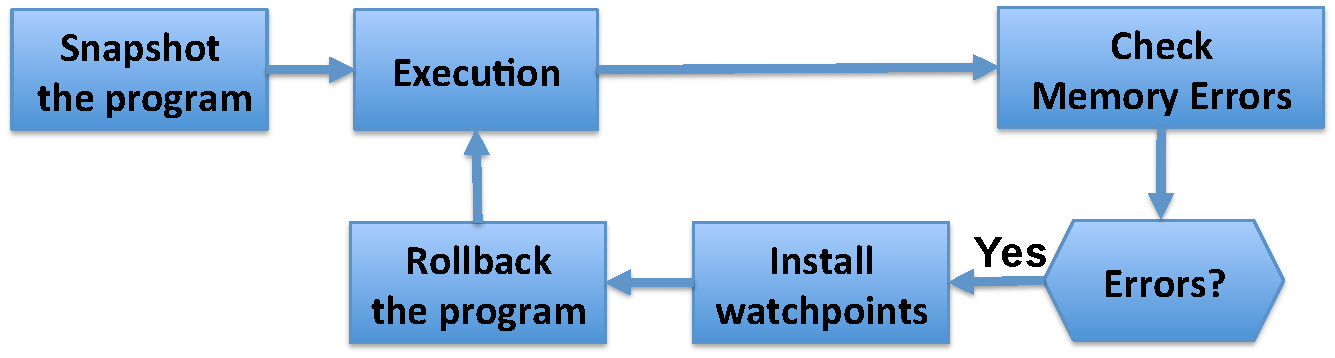
\includegraphics[width=5.4in]{fig/stopgapoverview2}
\caption{Overview of \stopgap{}
\label{fig:stopgapoverview}}
}
\end{figure}

% What is the rollback mechanism
\subsection{Re-execution of A Program}
\label{sec:re-execute}
\stopgap{} targets to locate those overflows precisely using the re-execution,
thus it is important for \stopgap{} to repeat the initial execution:
those overflows and races happening in the initial execution should happen exactly the same in
the re-execution phase, on the same addresses and with the same behavior.
In order to achieve this target, 
we are planning to utilize the \dthreads{} framework for determinism support.  

% What is the watch point mechanism
\subsection{Watch Point Mechanism}
\label{sec:watchpoint}

Watch point mechanism is using hardware debug registers to watch the memory accesses on
some specific addresses. Some previous works have used this mechanism 
for their specific targets \cite{fastboundschecking}. 
Debug register hardware is universally supported by most if not all existing CPUs, such as
X86 and X86-64 architecture, PowerPC, MIPS, ARM, etc. 
Generally, this watch point technique can support the memory watching efficiently: whenever
a memory access matches one of those debugging address, the user can be notified by an exception.
% What is the basic idea of \stopgap{}.

\section{Buffer Overflow}
Those existing mechanisms to find out buffer overflow problems either can not pinpoint the origins of
problems precisely or their performance overhead is too high to be deployed. 
Those traditional approaches pinpointting the origins of problems should 
check every memory access in order to capture those accesses beyond the scope of 
current memory block. 
If a buffer overflow is found, the program will be stopped immediately 
so that user can find out where the problem occurs.
Thus, this kind of approach is also called as ``stop-and-report'' approach here. 

However, ``stop-and-report'' approach introduces significant performance overhead by 
checking every memory access,  
preventing their usage in actual deployed environment. 
We propose to utilize the \stopgap{} mechanism (described in the above section) 
to detect buffer overflows and underflows efficiently. 

In order to detect those overflows, \stopgap{} puts one guard zone before and 
one after each heap object. \stopgap{} initializes all guard zones to a pre-known special 
value when a heap object is allocated.
When buffer overflow occurs, values of guard zones must be changed to a different value.
By detecting the changes of guard zones, \stopgap{} can detect the buffer overflows. 
%Since \stopgap{} greately reduces the number of checkings, the overhead
%is expected to be largely amortized over a long execution time.
%\stopgap{} can report more information than the traditional stop-and-report approach:
%\stopgap{} can provide the whole access sequence
%on some specific addresses, which can help to identify the actual
%problems in the complex systems.
Same as the mechanisms to locate the write-write races, \stopgap{} only checks overflows 
in the end of a program or at synchronization boundries, hoping to greately reduce
the overhead.  
\stopgap{} also utilizes the rollback mechnism and watch point mechanism to find
the origins of overflows precisely.

\subsection{Preliminary Results}
We have finished a practical buffer overflow detection tool for single-threaded program, which only
introduces minor performance overhead (about 5\%), much lower than the state-of-the-art technique.
The state-of-the-art tool to detect the buffer overflow problem,
AddressSanitizer from \texttt{Google}, introduces about 26\% performance overhead.

% What is the challenge here?
\section{Schedule and Delieverables}

The proposed timeline for this thesis is as follows:

\begin{table}[ht]
\centering
\begin{tabular}{ l r}
Implementing the basic machanism of \stopgap{} & March 2013 \\ 
Evaluating the performance and effectiveness & May 2013 \\
Improving the performance and effectiveness & June 2013 \\
Thesis chapter drafts & May 2013 \\ 
Paper submitted to ASPLOS & July 2013 \\
Thesis defense  & Summer 2013\\
Graduate & Summer 2013 \\
\end{tabular}
{\label{table:timeline}}
\end{table}

For this thesis work, ideally, a paper would be submitted to ASPLOS conference in July 2013. 
Corresponding code will be publicize on GitHub, so that people can utilize the software
derived from this thesis work
to detect the race conditions and buffer overflows in multithreaded programs.
